% SC4002 --- Chapter 8: Generation --- Sampling, RLHF, and Evaluation (0->100 ground-up)
\chapter{Generation: Sampling, Alignment, and Evaluation}
\label{ch:generation}

\begin{quote}
\emph{``A language model knows how to continue; generation decides \emph{which} continuation to show, and evaluation decides whether it was any good.''} --- This chapter turns next-token probabilities into text and judgement.
\end{quote}

\noindent\fbox{\parbox{\dimexpr\linewidth-2\fboxsep-2\fboxrule}{%
\textbf{From zero: no generation background assumed.} We start from a model that outputs a distribution over the next word and ask: why picking the best word every time fails, how to inject controlled randomness, how to align outputs to human preferences with RLHF, and how BLEU/ROUGE score generated text. Every formula is motivated by a picture first.}}
\vspace{0.4em}

\section*{Learning Outcomes}
After this chapter you will be able to:
\begin{enumerate}[label=(L\arabic*)]
    \item explain why greedy decoding is locally optimal but globally suboptimal and repetitive;
    \item write sampling formulas for temperature, top-$k$, and top-$p$ (nucleus) and trade diversity vs.\ quality;
    \item describe the RLHF pipeline (SFT, reward model, PPO) and the DPO shortcut;
    \item compute BLEU with n-gram precision, brevity penalty, and ROUGE recall including ROUGE-L;
    \item implement nucleus sampling and BLEU in Python and choose metrics for a task.
\end{enumerate}

% ============================================================
\section{From Probabilities to Text: Why Greedy Fails}
\label{sec:greedy-intuition}
\paragraph{Intuition.} A language model gives $P(y_t \mid y_{<t}, x)$ for every vocab item. Greedy decoding picks $\hat{y}_t = \arg\max_y P(y\mid y_{<t})$ at each step. This is like always taking the steepest uphill step: you reach a local peak but miss the mountain. Worse, language is multimodal: after ``I love'', both ``cats'' and ``dogs'' are good; greedy commits to one path and cannot backtrack if later words become awkward. Empirically, greedy produces bland, repetitive text (``I think I think I think'') because high-frequency phrases dominate each local choice.

\paragraph{Formal setup.} Let logits $\mathbf{z}\in\mathbb{R}^{|V|}$ produce $P(y=i\mid \text{ctx})=\text{softmax}(\mathbf{z})_i$. Greedy decodes
\begin{equation}
y_t^* = \arg\max_{i} \log P(y_t=i\mid y_{<t}, x), \quad \mathbf{y}^*=(y_1^*,\dots,y_T^*).
\end{equation}
Beam search generalises greedy: keep top-$B$ hypotheses, scoring $\sum_{t}\log P(y_t\mid y_{<t})$. With $B=1$ it is greedy; with larger $B$ it approximates $\arg\max_{\mathbf{y}}P(\mathbf{y}\mid x)$ but still maximises likelihood, not human preference, and remains deterministic.

\paragraph{Example.} Prompt: ``The cat sat on the''. Model: $P(\text{mat}\mid\cdot)=0.4$, $P(\text{roof}\mid\cdot)=0.35$, $P(\text{chair}\mid\cdot)=0.25$. Greedy picks ``mat'' every time, so 100 continuations are identical. A human wants variety: sometimes roof, sometimes chair, sometimes mat.

% ============================================================
\section{Sampling: Temperature, Top-$k$, Top-$p$}
\label{sec:sampling}
\paragraph{Intuition.} Sampling treats the distribution as a menu: temperature sharpens or flattens it, top-$k$ keeps only $k$ dishes, top-$p$ keeps enough dishes to cover $p$ of the appetite. All aim to balance \emph{quality} (stay on high-probability words) and \emph{diversity} (allow surprises).

\paragraph{Temperature scaling.} Divide logits by $\tau>0$ before softmax:
\begin{equation}
P_\tau(y=i\mid\text{ctx}) = \frac{\exp(z_i/\tau)}{\sum_j \exp(z_j/\tau)}.
\label{eq:temperature}
\end{equation}
$\tau\to 0$ sharpens to argmax (one-hot); $\tau=1$ is the original; $\tau>1$ flattens toward uniform. Low $\tau$ is safe but dull; high $\tau$ is creative but incoherent.

\paragraph{Top-$k$ and nucleus (top-$p$).} Let sorted $P_{(1)}\ge P_{(2)}\ge\cdots$. Top-$k$ keeps $\mathcal{V}_k=\{i: \text{rank}(i)\le k\}$ and renormalises:
\begin{equation}
P^{(k)}_i = \frac{P_i\cdot\mathbf{1}[i\in\mathcal{V}_k]}{\sum_{j\in\mathcal{V}_k}P_j}.
\end{equation}
Top-$p$ (nucleus) keeps the \emph{smallest} set with cumulative mass $\ge p$:
\begin{equation}
\mathcal{V}_p = \text{smallest } S \text{ s.t. } \sum_{i\in S} P_{(i)}\ge p,\quad P^{(p)}_i=\frac{P_i\cdot\mathbf{1}[i\in\mathcal{V}_p]}{\sum_{j\in\mathcal{V}_p}P_j}.
\label{eq:topp}
\end{equation}
Fixed $k$ wastes capacity when the distribution is peaked (top-1 suffices) and truncates too aggressively when flat; $p$ adapts: keep 2 words when confident, 50 when uncertain. Fig.~\ref{fig:temperature} visualises all three.

\begin{figure}[h]
\centering
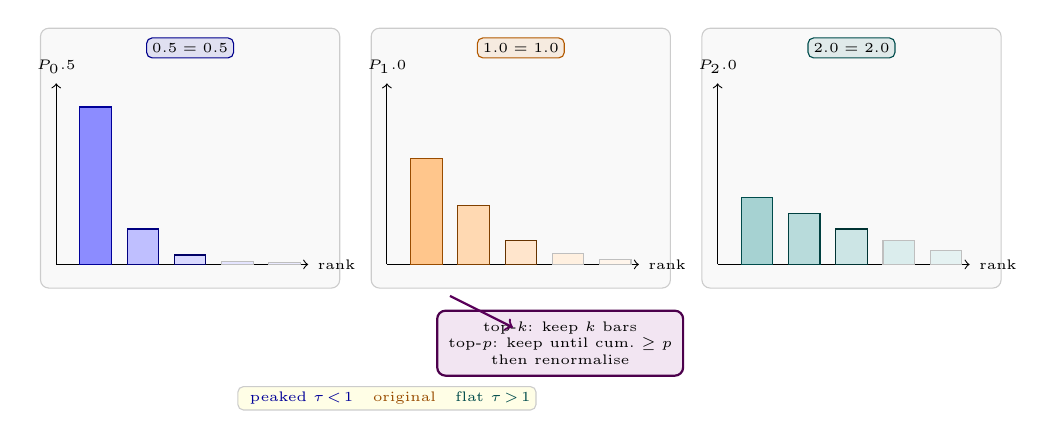
\begin{tikzpicture}[font=\scriptsize]
% --- three temperature panels ---
\foreach \idx/\tau/\col in {0/0.5/blue!55!black,1/1.0/orange!70!black,2/2.0/teal!60!black} {
  \begin{scope}[shift={(\idx*4.2,0)}]
    \draw[fill=gray!5, rounded corners=3pt, draw=gray!40] (-0.2,-0.3) rectangle (3.6,3.0);
    \node[font=\tiny, fill=\col!12, draw=\col, rounded corners=2pt, inner sep=2pt] at (1.7,2.75) {$\tau=\tau$};
    \draw[->] (0,0) -- (3.2,0) node[right, font=\tiny] {rank};
    \draw[->] (0,0) -- (0,2.3) node[above, font=\tiny] {$P_\tau$};
    % bars -- different shapes
    \ifnum\idx=0
      \fill[blue!45, draw=blue!60!black] (0.3,0) rectangle (0.7,2.0);
      \fill[blue!25, draw=blue!50!black] (0.9,0) rectangle (1.3,0.45);
      \fill[blue!15, draw=blue!40!black] (1.5,0) rectangle (1.9,0.12);
      \fill[blue!10, draw=gray!50] (2.1,0) rectangle (2.5,0.04);
      \fill[blue!8, draw=gray!50] (2.7,0) rectangle (3.1,0.02);
    \fi
    \ifnum\idx=1
      \fill[orange!45, draw=orange!60!black] (0.3,0) rectangle (0.7,1.35);
      \fill[orange!30, draw=orange!50!black] (0.9,0) rectangle (1.3,0.75);
      \fill[orange!20, draw=orange!40!black] (1.5,0) rectangle (1.9,0.30);
      \fill[orange!12, draw=gray!50] (2.1,0) rectangle (2.5,0.14);
      \fill[orange!8, draw=gray!50] (2.7,0) rectangle (3.1,0.06);
    \fi
    \ifnum\idx=2
      \fill[teal!35, draw=teal!60!black] (0.3,0) rectangle (0.7,0.85);
      \fill[teal!28, draw=teal!50!black] (0.9,0) rectangle (1.3,0.65);
      \fill[teal!20, draw=teal!40!black] (1.5,0) rectangle (1.9,0.45);
      \fill[teal!14, draw=gray!50] (2.1,0) rectangle (2.5,0.30);
      \fill[teal!10, draw=gray!50] (2.7,0) rectangle (3.1,0.18);
    \fi
  \end{scope}
}
% top-k / top-p annotation
\node[draw=violet!60!black, thick, fill=violet!10, rounded corners=3pt, inner sep=4pt, font=\tiny, align=center] at (6.4,-1.0) {top-$k$: keep $k$ bars\\top-$p$: keep until cum.~$\ge p$\\then renormalise};
\draw[->, violet!70!black, thick] (5.0,-0.4) -- (5.8,-0.8);
\node[font=\tiny, fill=yellow!10, draw=gray!40, rounded corners=2pt, inner sep=2pt] at (4.2,-1.7) {\textcolor{blue!60!black}{$\blacksquare$ peaked $\tau\!<\!1$} \ \textcolor{orange!60!black}{$\blacksquare$ original} \ \textcolor{teal!60!black}{$\blacksquare$ flat $\tau\!>\!1$}};
\end{tikzpicture}
\caption{Temperature scaling and truncation. Low $\tau$ peaks on the top token (near-greedy); high $\tau$ spreads mass. Top-$k$ cuts after $k$ ranks regardless of shape; top-$p$ cuts when cumulative mass reaches $p$, adapting to peaked vs.\ flat distributions.}
\label{fig:temperature}
\end{figure}

% ============================================================
\section{Aligning to Humans: RLHF and DPO}
\label{sec:rlhf}
\paragraph{Intuition.} Likelihood rewards fluent text, not helpful or harmless text. Humans prefer answers that are truthful, concise, and refuse harmful requests, but the pre-training corpus contains all styles. RLHF teaches the model \emph{which} fluent continuations humans actually want by learning a reward function from comparisons and then optimising against it.

\paragraph{RLHF pipeline.} Three stages (Fig.~\ref{fig:rlhf}):
\begin{enumerate}[label=\arabic*., leftmargin=1.4em, itemsep=0.2em, topsep=0.2em]
    \item \textbf{SFT}: fine-tune base LM on high-quality demonstrations $(x, y^\star)$ with cross-entropy.
    \item \textbf{Reward model (RM)}: collect human preference pairs $(x, y_w, y_l)$ where $y_w\succ y_l$. Train $r_\phi(x,y)$ with Bradley--Terry loss:
    \begin{equation}
    \mathcal{L}_{\text{RM}}=-\mathbb{E}_{(x,y_w,y_l)}\!\left[\log\sigma\!\big(r_\phi(x,y_w)-r_\phi(x,y_l)\big)\right].
    \label{eq:rm-loss}
    \end{equation}
    \item \textbf{RL (PPO)}: treat LM $\pi_\theta$ as policy, maximise
    \begin{equation}
    J(\theta)=\mathbb{E}_{x\sim\mathcal{D},\,y\sim\pi_\theta(\cdot\mid x)}\!\left[r_\phi(x,y)\right]-\beta\,\text{KL}\!\left[\pi_\theta\,\|\,\pi_{\text{SFT}}\right],
    \label{eq:ppo-obj}
    \end{equation}
    via clipped PPO to stay near SFT. KL penalty prevents reward hacking (gibberish that fools $r_\phi$).
\end{enumerate}

\paragraph{DPO intuition.} PPO is heavy (rollouts, value network). DPO observes that the optimal policy for Eq.~\eqref{eq:ppo-obj} satisfies $r^\star\propto\log\frac{\pi^\star}{\pi_{\text{ref}}}$; substitute into Eq.~\eqref{eq:rm-loss} to train $\pi_\theta$ \emph{directly} on preferences:
\begin{equation}
\mathcal{L}_{\text{DPO}}=-\mathbb{E}\!\left[\log\sigma\!\left(\beta\log\frac{\pi_\theta(y_w\mid x)}{\pi_{\text{ref}}(y_w\mid x)}-\beta\log\frac{\pi_\theta(y_l\mid x)}{\pi_{\text{ref}}(y_l\mid x)}\right)\right].
\end{equation}
No reward model, no sampling loop; DPO is supervised learning on pairs with an implicit KL.

\begin{figure}[h]
\centering
\begin{tikzpicture}[
  box/.style={rectangle, rounded corners=3pt, thick, minimum width=2.6cm, minimum height=0.9cm, font=\scriptsize, align=center},
  arr/.style={-{Latex[length=2.4mm]}, thick, color=gray!70!black}
]
\node[box, fill=blue!14, draw=blue!60!black] (sft) at (0,0) {1. SFT\\{\tiny fine-tune on demos}\\$\pi_{\text{SFT}}$};
\node[box, fill=orange!15, draw=orange!70!black] (rm) at (4.0,0) {2. Reward Model\\{\tiny $r_\phi(x,y)$ from}\\{\tiny $y_w\succ y_l$}};
\node[box, fill=green!15, draw=green!55!black] (ppo) at (8.0,0) {3. PPO / DPO\\{\tiny optimise $\pi_\theta$}\\{\tiny vs.\ $r_\phi$ + KL}};
\node[box, fill=violet!12, draw=violet!60!black, minimum width=2.2cm] (human) at (4.0,2.0) {Humans\\{\tiny rank $y_w\succ y_l$}};
\draw[arr, blue!60!black] (sft) -- (rm) node[midway, above, font=\tiny, fill=white, inner sep=1pt] {init};
\draw[arr, orange!70!black] (rm) -- (ppo) node[midway, above, font=\tiny, fill=white, inner sep=1pt] {reward};
\draw[arr, violet!60!black] (human) -- (rm) node[midway, right, font=\tiny] {pairs};
\draw[arr, green!55!black, dashed] (rm.east) -- ++(0.6,0.9) -- ++(-8.6,0) -- (sft.north) node[pos=0.5, above, font=\tiny, fill=yellow!10, rounded corners=2pt, inner sep=2pt] {KL anchor $\pi_{\text{SFT}}$};
\node[font=\tiny, fill=yellow!8, draw=gray!40, rounded corners=2pt, inner sep=3pt] at (4.0,-1.15) {\textcolor{blue!60!black}{$\blacksquare$ policy} \ \textcolor{orange!70!black}{$\blacksquare$ reward} \ \textcolor{green!55!black}{$\blacksquare$ RL} \ \textcolor{violet!60!black}{$\blacksquare$ human}};
\end{tikzpicture}
\caption{RLHF pipeline. SFT gives a helpful base; humans provide preference pairs to train a reward model $r_\phi$; PPO (or DPO) pushes $\pi_\theta$ to maximise $r_\phi$ while staying close to $\pi_{\text{SFT}}$ via KL. DPO collapses steps 2--3 into one loss.}
\label{fig:rlhf}
\end{figure}

% ============================================================
\section{Evaluation: BLEU and ROUGE}
\label{sec:bleu-rouge}
\paragraph{Intuition.} How to score a generated sentence against references? Count overlapping word chunks ($n$-grams). Precision asks ``of what you wrote, how much was correct?'' Recall asks ``of what was expected, how much did you cover?'' BLEU is precision-oriented (for translation); ROUGE is recall-oriented (for summarisation).

\paragraph{BLEU.} For candidate $c$ (length $c$) and reference $r$ (length $r$, closest length), modified $n$-gram precision $p_n$ clips counts to the max in any reference. With $N=4$, $w_n=1/N$:
\begin{equation}
\text{BLEU}= \text{BP}\cdot\exp\!\Big(\sum_{n=1}^{N} w_n \log p_n\Big),\quad
\text{BP}=\begin{cases}1 & c>r\\ \exp(1-r/c) & c\le r\end{cases}
\label{eq:bleu}
\end{equation}
BP is the \emph{brevity penalty}: short candidates that cheat on precision are penalised. Geometric mean means one zero $p_n$ zeroes BLEU (smoothing variants fix this). Fig.~\ref{fig:bleu} shows clipping.

\paragraph{ROUGE.} ROUGE-$N$ is recall over $n$-grams (let $c_g{=}\text{count}_c(g)$, $r_g{=}\text{count}_r(g)$):
\begin{equation}
\text{ROUGE-N}=\frac{\sum_{g\in\text{ref}}\min(c_g,r_g)}{\sum_{g\in\text{ref}} r_g}.
\end{equation}
ROUGE-L uses longest common subsequence: with $\text{LCS}(c,r)$,
\begin{align}
R_{\text{LCS}}&=\frac{|\text{LCS}|}{|r|},\\
P_{\text{LCS}}&=\frac{|\text{LCS}|}{|c|},\\
F_{\text{LCS}}&=\frac{(1+\beta^2)RP}{R+\beta^2 P}.
\end{align}
LCS captures word order without fixing $n$. Both BLEU and ROUGE are string-overlap proxies and correlate imperfectly with human judgement.

\begin{figure}[h]
\centering
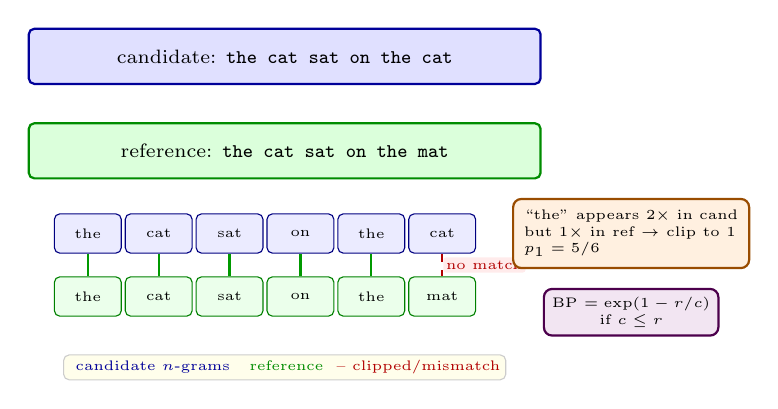
\begin{tikzpicture}[font=\scriptsize]
% candidate
\node[draw=blue!60!black, thick, fill=blue!12, rounded corners=2pt, minimum width=6.5cm, minimum height=0.7cm] (cand) at (3.4,2.4) {candidate: \texttt{the cat sat on the cat}};
\node[draw=green!55!black, thick, fill=green!14, rounded corners=2pt, minimum width=6.5cm, minimum height=0.7cm] (ref) at (3.4,1.2) {reference: \texttt{the cat sat on the mat}};
% n-gram boxes
\foreach \i/\w in {1/the,2/cat,3/sat,4/on,5/the,6/cat} {
  \node[draw=blue!50!black, fill=blue!8, rounded corners=2pt, minimum width=0.85cm, minimum height=0.5cm, font=\tiny] (c\i) at (0.9*\i,0.15) {\w};
}
\foreach \i/\w in {1/the,2/cat,3/sat,4/on,5/the,6/mat} {
  \node[draw=green!50!black, fill=green!8, rounded corners=2pt, minimum width=0.85cm, minimum height=0.5cm, font=\tiny] (r\i) at (0.9*\i,-0.65) {\w};
}
% matching lines
\draw[thick, green!60!black] (c1) -- (r1); \draw[thick, green!60!black] (c2) -- (r2);
\draw[thick, green!60!black] (c3) -- (r3); \draw[thick, green!60!black] (c4) -- (r4);
\draw[thick, green!60!black] (c5) -- (r5);
\draw[thick, red!70!black, dashed] (c6) -- (r6) node[midway, right, font=\tiny, fill=red!8, rounded corners=1pt, inner sep=1pt] {no match};
% clipped count note
\node[draw=orange!60!black, thick, fill=orange!12, rounded corners=3pt, font=\tiny, align=left, inner sep=4pt] at (7.8,0.15) {``the'' appears $2\times$ in cand\\but $1\times$ in ref $\to$ clip to 1\\$p_1 = 5/6$};
\node[draw=violet!60!black, thick, fill=violet!10, rounded corners=3pt, font=\tiny, align=center, inner sep=3pt] at (7.8,-0.85) {BP $=\exp(1-r/c)$\\if $c\le r$};
\node[font=\tiny, fill=yellow!8, draw=gray!40, rounded corners=2pt, inner sep=2pt] at (3.4,-1.55) {\textcolor{blue!60!black}{$\blacksquare$ candidate $n$-grams} \ \textcolor{green!55!black}{$\blacksquare$ reference} \ \textcolor{red!70!black}{-- clipped/mismatch}};
\end{tikzpicture}
\caption{BLEU $n$-gram matching with clipping. Candidate ``cat'' matches once; the second ``the'' is clipped because the reference has only one ``the'' after ``on''. Unmatched n-grams lower $p_n$; short candidates are further penalised by BP.}
\label{fig:bleu}
\end{figure}

\begin{lstlisting}[language=Python, caption={Nucleus (top-$p$) sampling and sentence-level BLEU with brevity penalty.}, label={lst:topp-bleu}]
import numpy as np
from collections import Counter

def nucleus_sampling(logits, p=0.9, temperature=1.0):
    """Sample one token from logits with temperature + top-p."""
    logits = np.array(logits) / max(temperature, 1e-9)
    # softmax
    e = np.exp(logits - logits.max())
    probs = e / e.sum()
    # sort descending
    idx = np.argsort(-probs)
    sorted_p = probs[idx]
    cumsum = np.cumsum(sorted_p)
    # keep smallest set with cumsum >= p
    cutoff = np.searchsorted(cumsum, p) + 1
    keep = idx[:cutoff]
    # renormalise
    filt = probs[keep] / probs[keep].sum()
    return int(np.random.choice(keep, p=filt))

# demo: peaked distribution
print(nucleus_sampling([3.0, 1.0, 0.2, 0.1], p=0.9, temperature=0.8))

def sentence_bleu(candidate, reference, N=4):
    """Toy BLEU without smoothing: candidate/reference are token lists."""
    c, r = len(candidate), len(reference)
    BP = 1.0 if c > r else np.exp(1 - r / max(c, 1))
    p_ns = []
    for n in range(1, N+1):
        cand_ngrams = Counter(tuple(candidate[i:i+n]) for i in range(c-n+1))
        ref_ngrams  = Counter(tuple(reference[i:i+n]) for i in range(r-n+1))
        overlap = sum(min(cand_ngrams[g], ref_ngrams[g]) for g in cand_ngrams)
        total = max(sum(cand_ngrams.values()), 1)
        p_ns.append(overlap / total)
    # geometric mean; 0 if any p_n == 0 (real BLEU smooths this)
    if min(p_ns) == 0:
        return 0.0, p_ns, BP
    score = BP * np.exp(sum(np.log(p) for p in p_ns) / N)
    return score, p_ns, BP

cand = "the cat sat on the cat".split()
ref  = "the cat sat on the mat".split()
print(sentence_bleu(cand, ref, N=2))  # (BLEU, [p1,p2], BP)
\end{lstlisting}
% ============================================================
\section{Chapter Notes}
Greedy/beam search and sampling are surveyed by Holtzman et al.\ (2020, nucleus sampling) and Fan et al.\ (2018, hierarchical stories). RLHF was scaled by Ouyang et al.\ (2022, InstructGPT) and Christiano et al.\ (2017); trust-region PPO is Schulman et al.\ (2017). DPO (Rafailov et al., 2023) removes the RL loop. BLEU is Papineni et al.\ (2002); ROUGE is Lin (2004). String overlap metrics miss semantics---learned metrics (BERTScore, COMET) and human evaluation remain essential.

% ============================================================
\section{Exercises}
\label{sec:ch08-exercises}
\begin{enumerate}[label=E8.\arabic*, leftmargin=*, itemsep=0.7em]
    \item \textbf{Temperature arithmetic.} Logits $[2,1,0]$ give $P\propto[e^2,e^1,1]$. Compute $P_{0.5},P_1,P_2$ via Eq.~\eqref{eq:temperature}. Which $\tau$ makes the top token exceed $0.9$? Explain why $\tau\to0$ recovers greedy and $\tau\to\infty$ recovers uniform.
    \item \textbf{Top-$k$ vs.\ top-$p$.} Distribution $P=[0.5,0.3,0.1,0.06,0.04]$. (a) What set does top-$k$ with $k=2$ keep and with what renormalised probs? (b) What set does top-$p$ with $p=0.85$ keep? (c) Give a peaked and a flat distribution where the two methods disagree sharply and argue which adapts better.
    \item \textbf{Reward model loss.} With $r_\phi(x,y_w)=1.2$, $r_\phi(x,y_l)=0.4$, compute $\mathcal{L}_{\text{RM}}$ from Eq.~\eqref{eq:rm-loss} and its gradient w.r.t.\ $\Delta=r_w-r_l$. What happens to the gradient when $\Delta\gg0$ vs.\ $\Delta\approx0$? Relate to DPO's implicit reward.
    \item \textbf{BLEU by hand.} Candidate ``the cat the cat'' (c=4) vs.\ reference ``the cat sat'' (r=3). Compute clipped $p_1,p_2$, BP, and BLEU-2 with $w_1=w_2=0.5$. Then compute ROUGE-1 recall and explain why BLEU penalises the repetition differently than ROUGE.
    \item \textbf{Build and critique.} Using the code in Listing~\ref{lst:topp-bleu}, (a) generate 5 samples from logits $[2,1.5,1,0.2]$ with $p=0.9,\tau=1$ vs.\ greedy, (b) compute BLEU-4 for candidates of length 3 vs.\ 10 against a length-8 reference to see BP in action, and (c) propose one failure mode of BLEU/ROUGE for dialogue and suggest a better evaluation.
\end{enumerate}
% End of Chapter 8
